\documentclass[../lab2.tex]{subfiles}

\begin{document}
    In questa configurazione i due host comunicano attraverso adattatori powerline,
    quindi l'informazione passa attraverso l'impianto elettrico.
    La velocita' di trasmissione cosi' come i protocolli utilizzati a questo livello
    non sono noti, quindi si ipotizza l'uso del protocollo ethernet e si cerca di 
    stimare la velocita' tra i due adattatori powerline.
    Abbiamo notato utlizzando il comando ethtool che la velocita' massima negoziata
    tra il router e gli host era di 100 Mb/s

    \begin{center}
        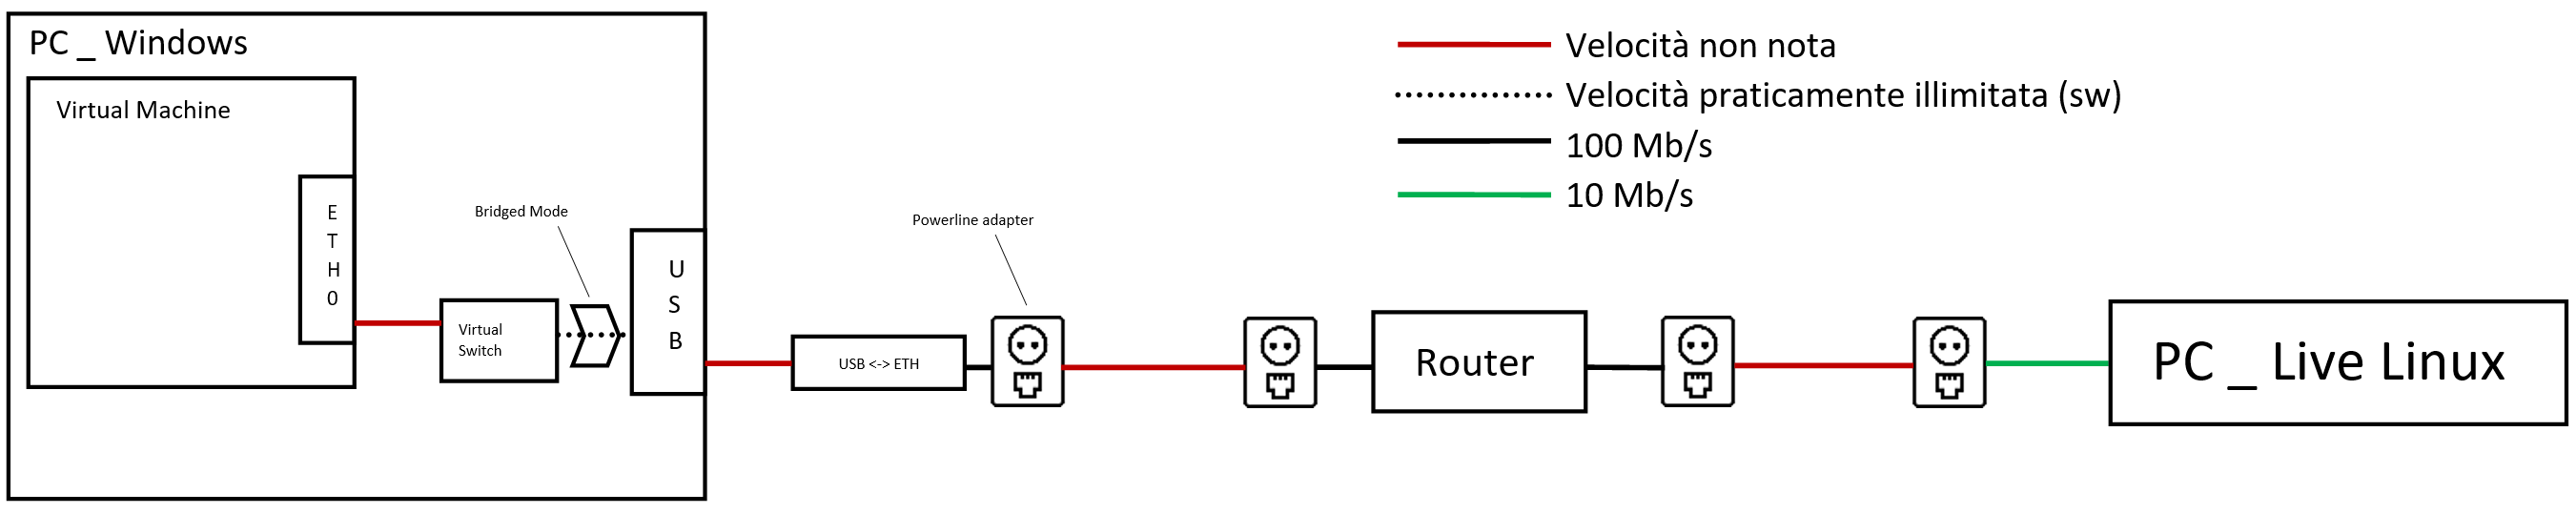
\includegraphics[width=1\linewidth]{conf4.png}
    \end{center}
\end{document}